\section{Netzebenen}
    \begin{center}
        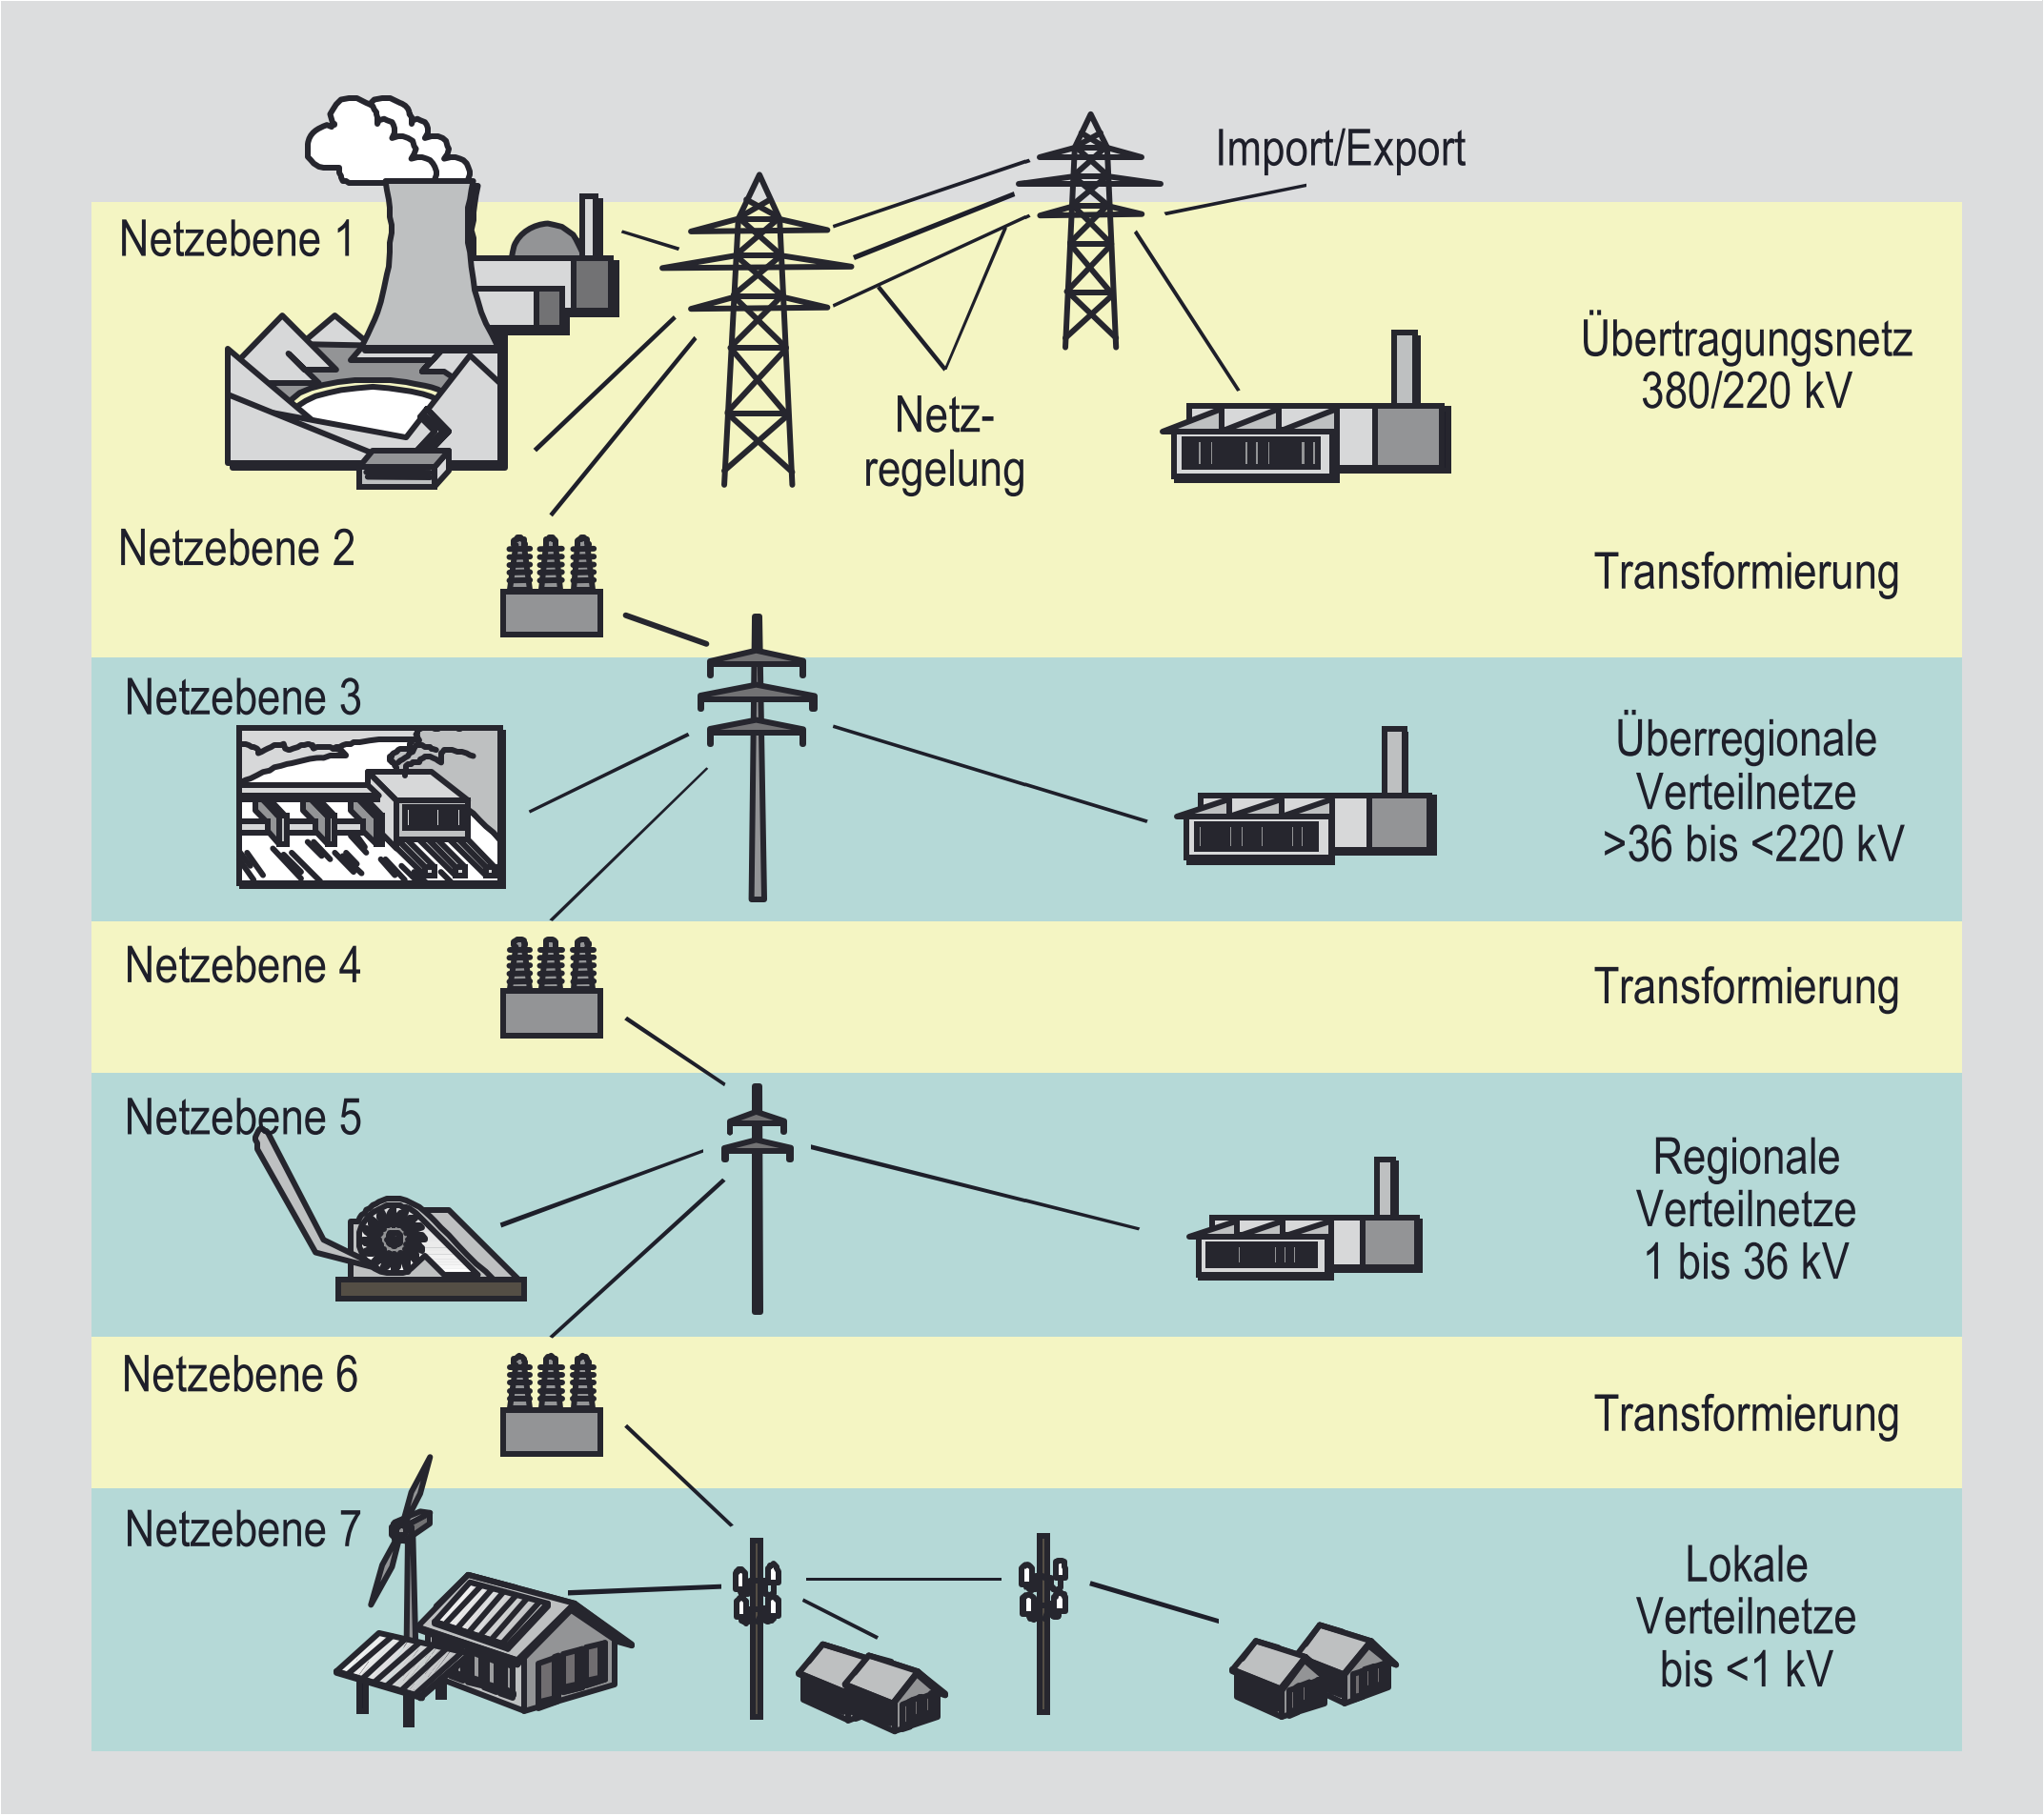
\includegraphics[width=0.95\columnwidth, align=c]{images/Netzebenen_1.png}
    \end{center}

    \begin{center}
        \begin{tabular}{>{\bfseries}l l l}
            \toprule
            Spannungsebene & Spannungsbereich & Leistung \\
            \midrule
            Höchstspannung   & 380 kV, 220 kV         & > 300 MVA \\
            Hochspannung     & 150 kV bis 50 kV       & < 100 MVA \\
            Mittelspannung   & 36 kV bis 6 kV         & < 30 MVA \\
            Niederspannung   & 0{,}4 kV               & < 1 MVA \\
            \bottomrule
        \end{tabular}
    \end{center}

\subsection{NE1: Übertragungsnetz (380\,kV, 220\,kV)}
    \begin{minipage}[t]{0.5\columnwidth}
        \begin{itemize}
            \item \textbf{Zweck}
            \begin{itemize}
                \item Abtransport der großen KW-Leistungen (typ. > 300\,MVA)
                \item Versorgung der Verteilnetze
                \item Weiträumiger Energietransport
                \item Internat. Verbundbetrieb, Energieaustausch
            \end{itemize}
        \end{itemize}
    \end{minipage}%
    \hfill
    \begin{minipage}[t]{0.49\columnwidth}
        \begin{itemize}
            \item \textbf{Ausdehnung:} national, international
            \item \textbf{Topologie:} (stark) vermaschtes Netz
            \item \textbf{Technologie:} fast nur Freileitungen
        \end{itemize}
    \end{minipage}

\subsubsection{Schweizer Stromübertragungsnetz (Daten 2014)}
    \begin{center}
        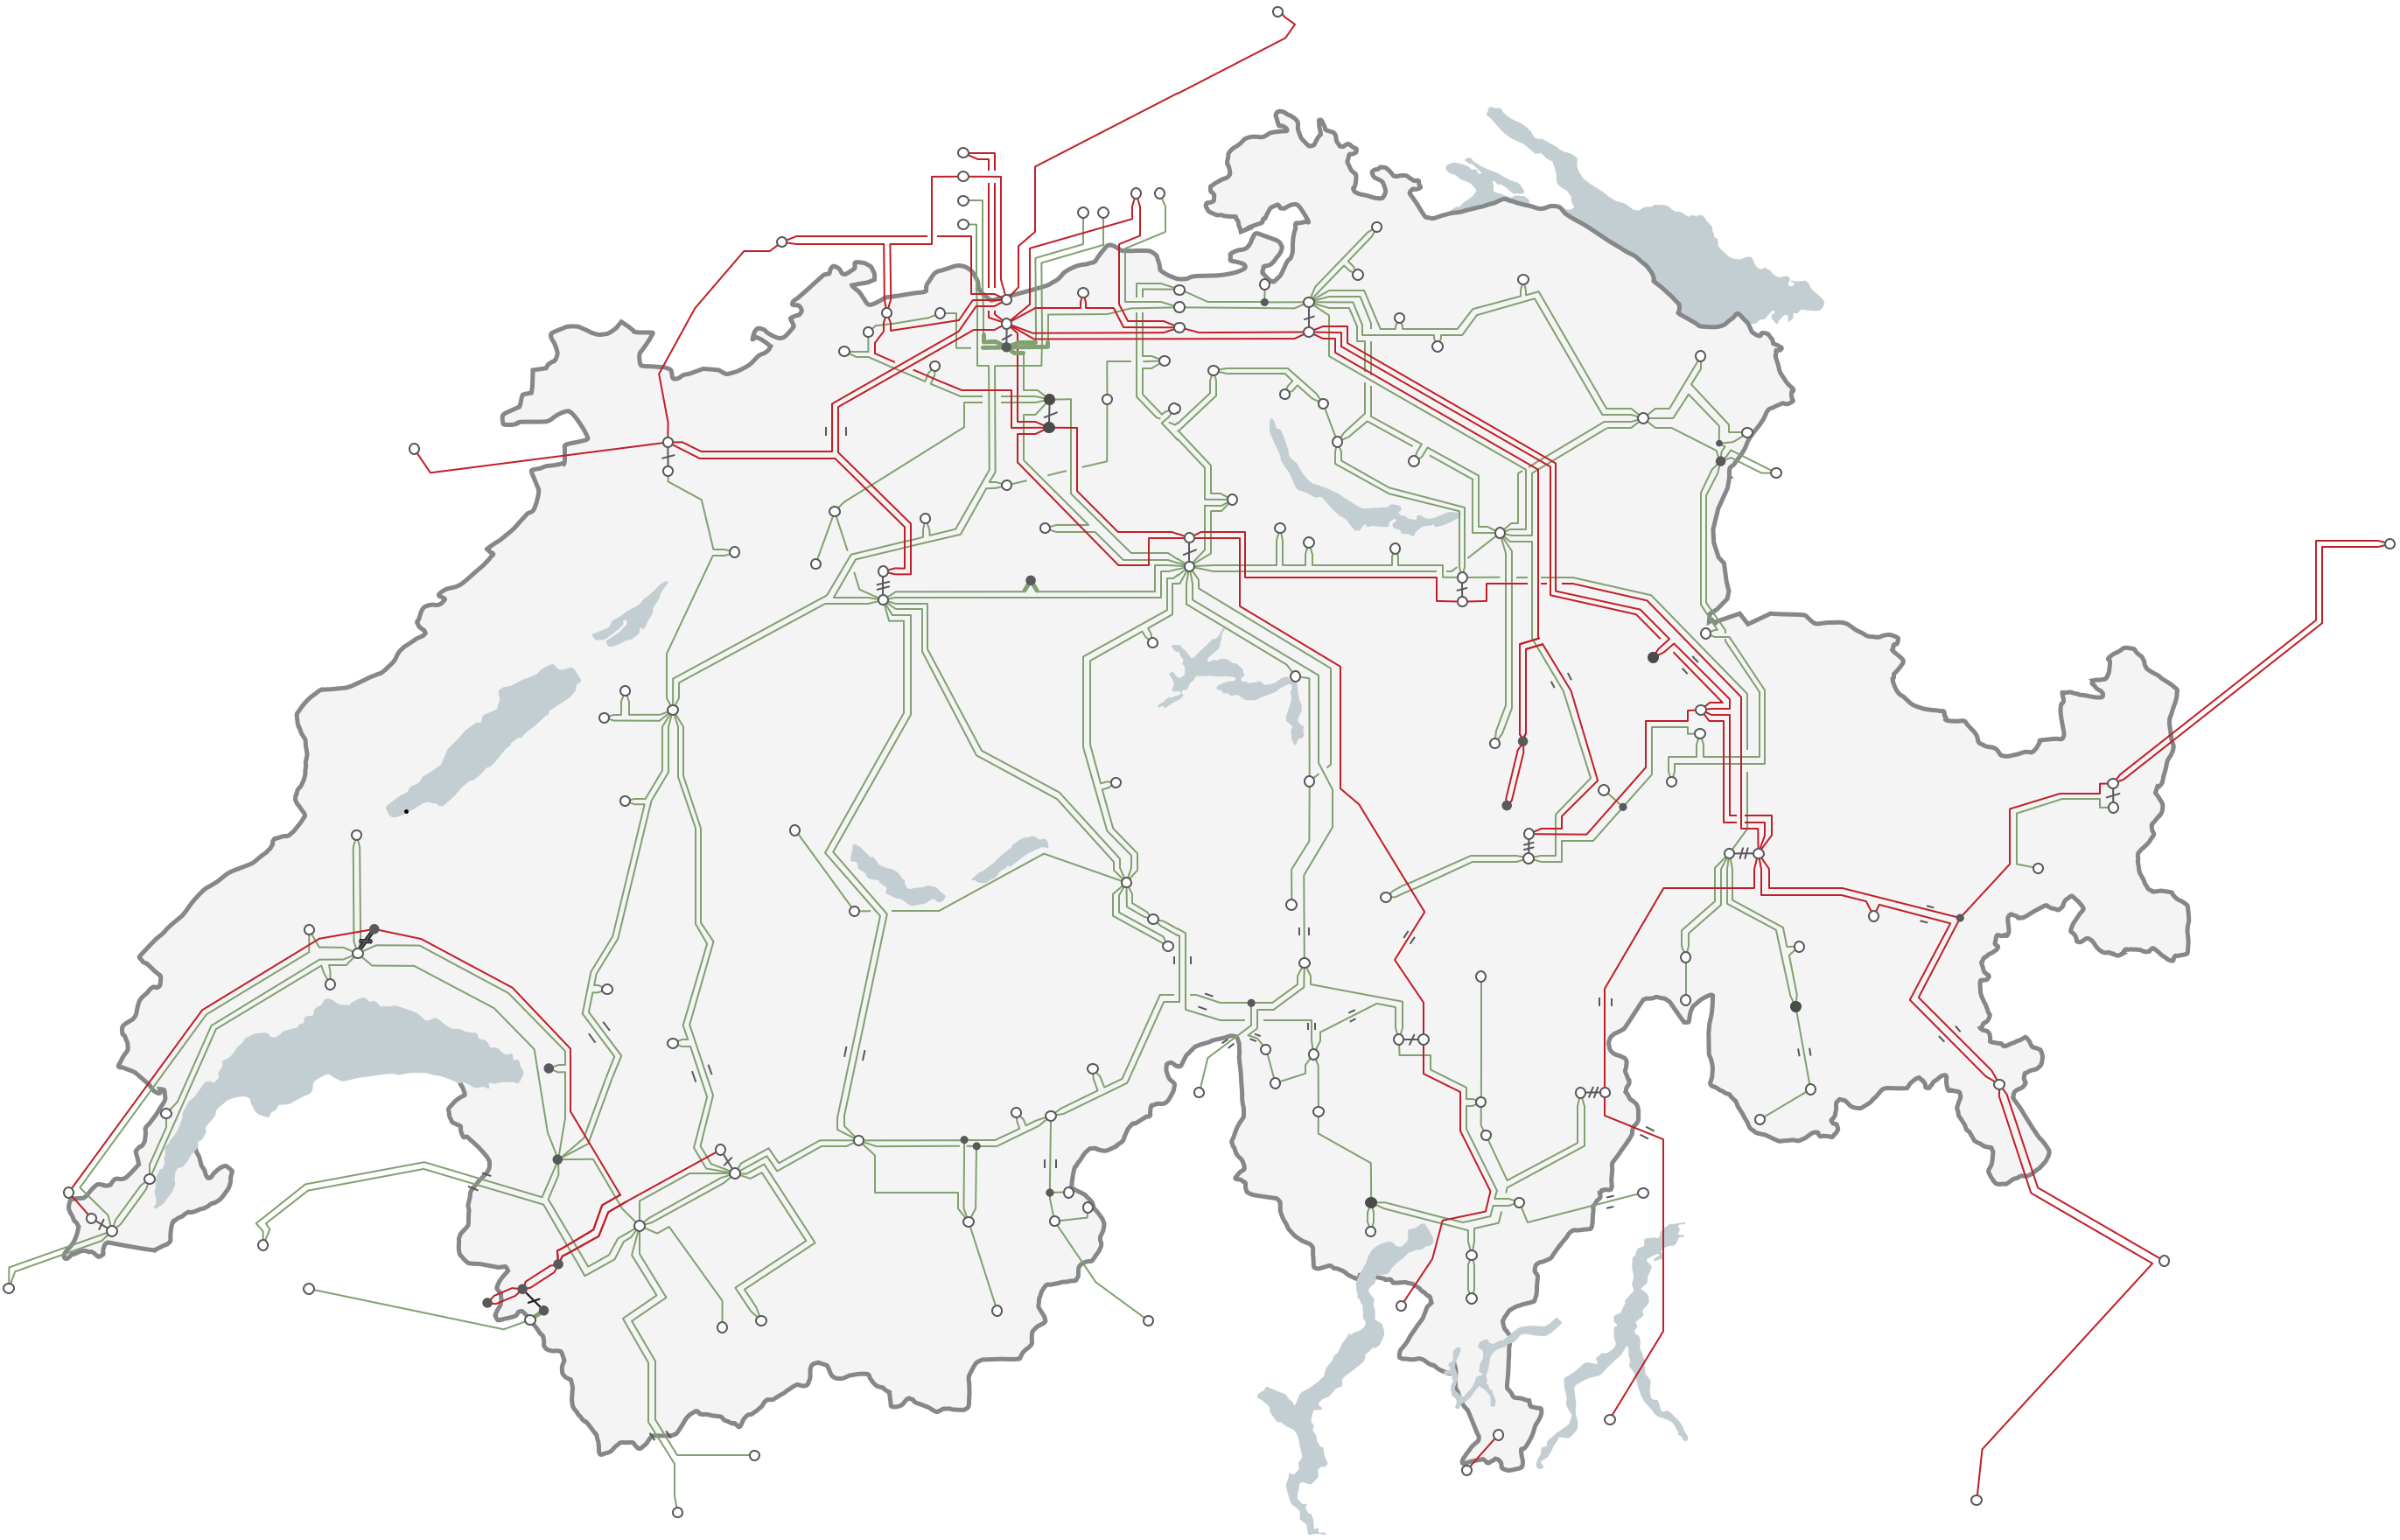
\includegraphics[width=0.95\columnwidth, align=c]{images/Schweizer_übertragungsnetz.png}
    \end{center}

    \begin{itemize}
        \item Gesamtlänge Übertragungsnetz Inland: 6700 km
        \begin{itemize}
            \item Länge 380\,kV: 1780 km
            \item Länge 220\,kV: 4920 km
        \end{itemize}
        
        \item Gesamtzahl Leitungen im Übertragungsnetz: 246
        \begin{itemize}
            \item Leitungen 380\,kV: 48
            \item Leitungen 220\,kV: 198
        \end{itemize}
        
        \item Anzahl Netzübergänge in das Ausland: 41
    \end{itemize}

\subsubsection{Entso-E}
    \begin{minipage}[t]{0.39\columnwidth}
        \textbf{Koordination von:}
        \begin{itemize}
            \item Systembetrieb
            \item Marktlösungen
            \item Systementwicklung
        \end{itemize}
    \end{minipage}
    \hfill
    \begin{minipage}[t]{0.6\columnwidth}
        \centering \vspace{-0.7\baselineskip}
        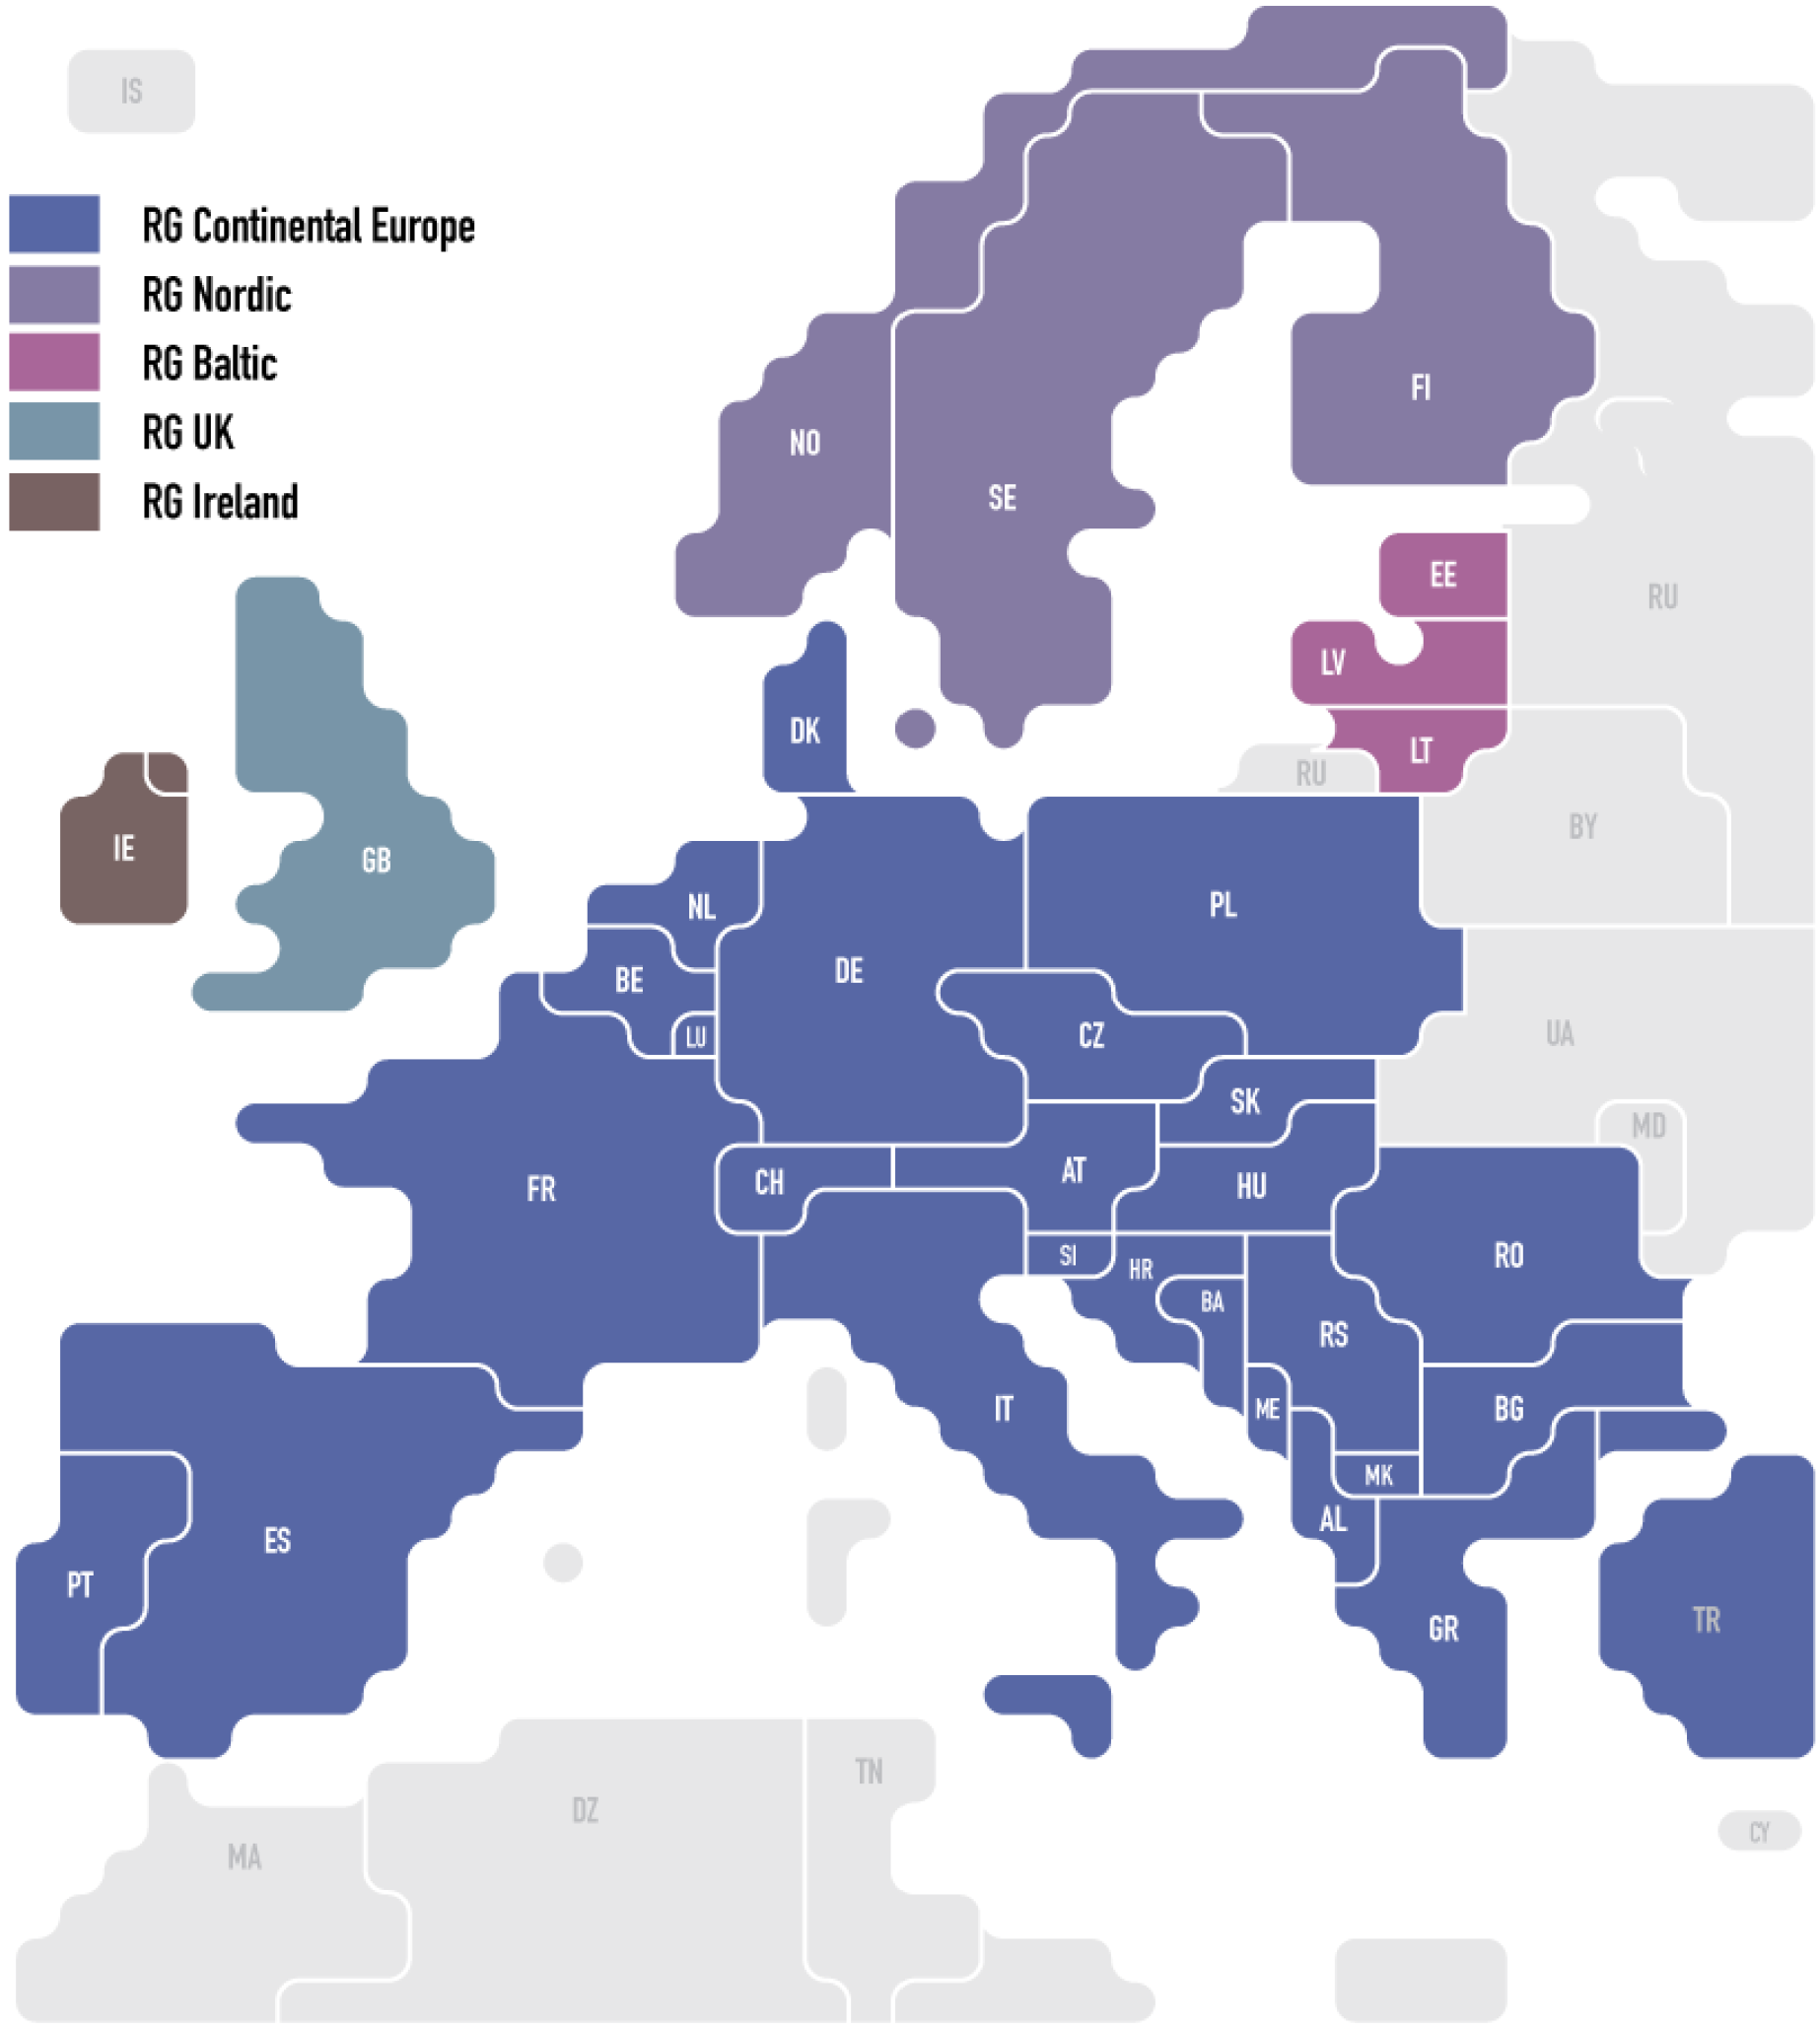
\includegraphics[width=0.8\textwidth]{images/Entso_E.png}
    \end{minipage}%

    % \begin{center}
    %     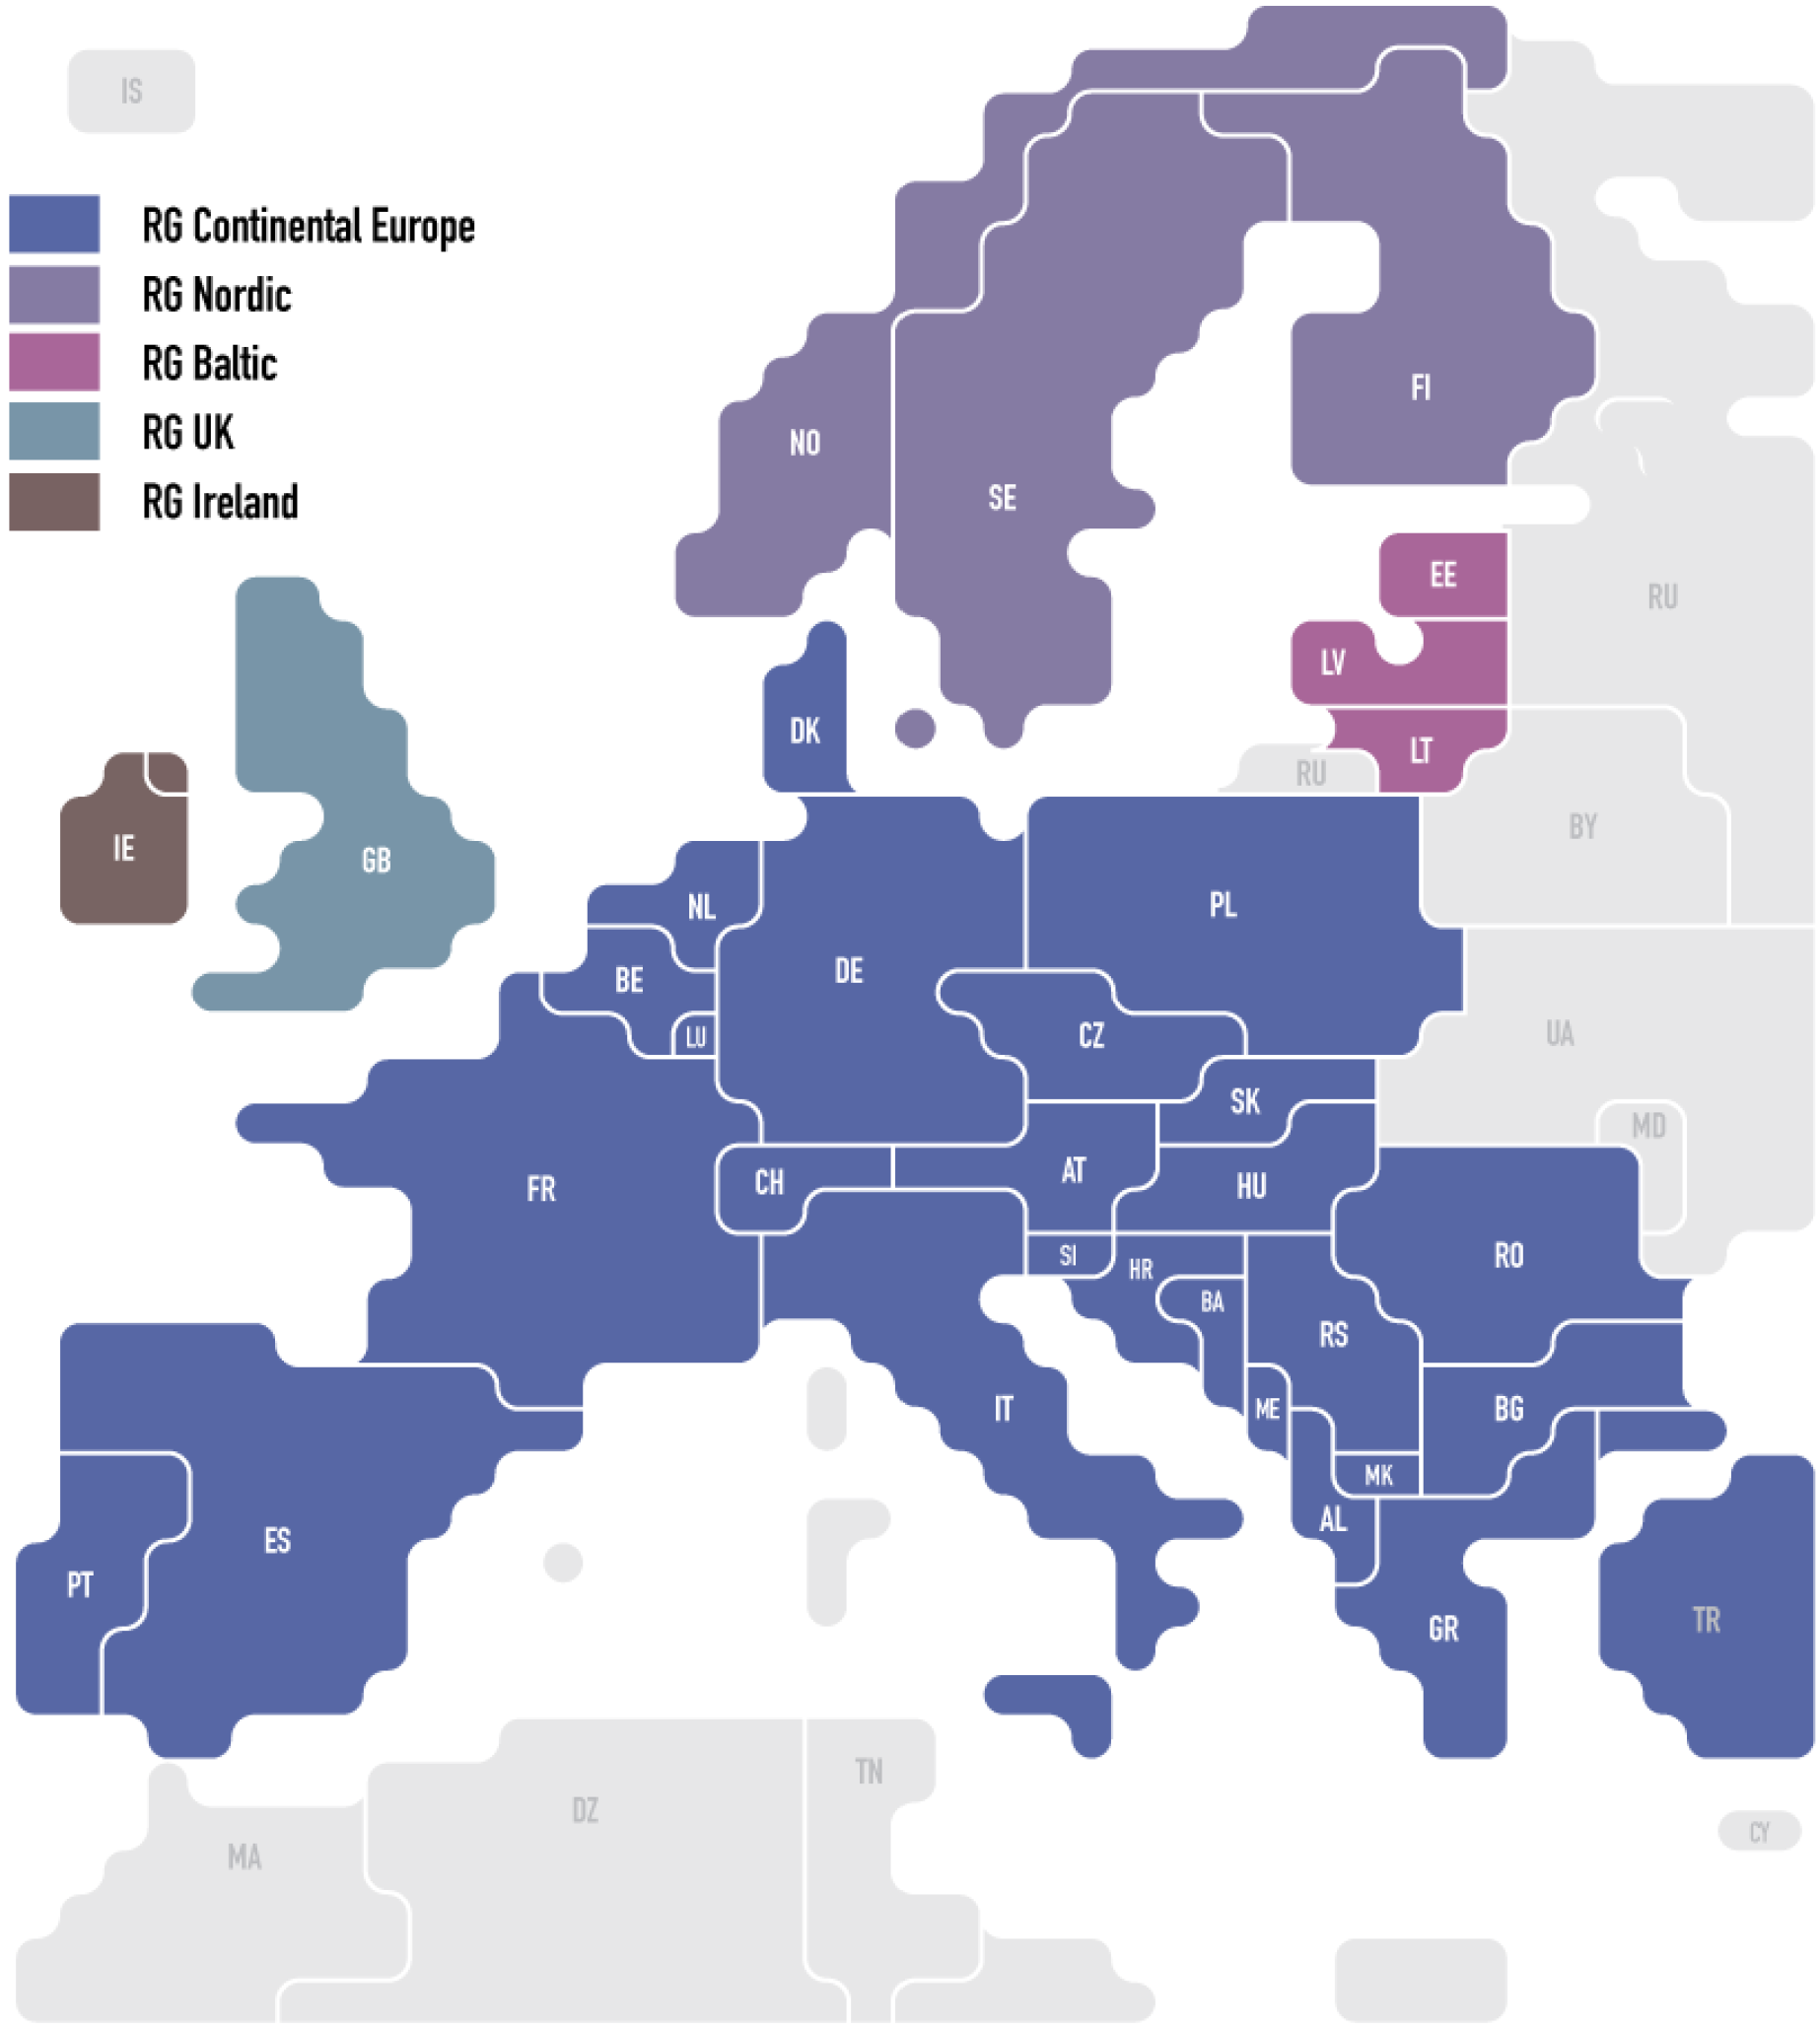
\includegraphics[width=0.75\columnwidth, align=c]{images/Entso_E.png}
    % \end{center}

    % \begin{itemize}
    %     \item koordinierter Systembetrieb
    %     \item koordinierte Marktlösungen
    %     \item koordinierte Systementwicklung
    % \end{itemize}

\subsection{NE3: Überregionales Verteilnetz (150, 132, 60\,kV)}
    \begin{minipage}[t]{0.5\columnwidth}
        \begin{itemize}
            \item \textbf{Zweck}
            \begin{itemize}
                \item Abtransport mittlerer Kraftwerksleistungen (typ. 100\,MVA)
                \item Anschluss großer Industriekunden
                \item Überregionale Verteilung
            \end{itemize}
        \end{itemize}
    \end{minipage}%
    \hfill
    \begin{minipage}[t]{0.49\columnwidth}
        \begin{itemize}
            \item \textbf{Ausdehnung:} mehrere Kantone
            \item \textbf{Topologie:} (leicht) vermascht oder Ring
            \item \textbf{Technologie:} vorwiegend Freileitungen
        \end{itemize}
    \end{minipage}
    % \begin{itemize}
    %     \item Zweck
    %     \begin{itemize}
    %         \item Abtransport mittlerer Kraftwerksleistungen (typ. 100 MVA)
    %         \item Anschluss großer Industriekunden
    %         \item Überregionale Verteilung
    %     \end{itemize}
    %     \item Ausdehnung: mehrere Kantone
    %     \item Topologie: (leicht) vermaschtes Netz oder Ringnetz
    %     \item Technologie: vorwiegend Freileitungen
    % \end{itemize}

\subsection{NE5: Verteilnetz (20, 10\,kV)}
    \begin{minipage}[t]{0.5\columnwidth}
        \begin{itemize}
            \item \textbf{Zweck}
            \begin{itemize}
                \item Abtransport kleiner Kraftwerksleistungen (< 30\,MVA)
                \item Anschluss von Industrie- und Gewerbekunden
                \item Regionale Verteilung
            \end{itemize}
        \end{itemize}
    \end{minipage}%
    \hfill
    \begin{minipage}[t]{0.49\columnwidth}
        \begin{itemize}
            \item \textbf{Ausdehnung:} Kanton, Tal
            \item \textbf{Topologie:} Ringnetz, Strahlennetz
            \item \textbf{Technologie:} Freileitungen und Kabel
        \end{itemize}
    \end{minipage}
    % \begin{itemize}
    %     \item Zweck
    %     \begin{itemize}
    %         \item Abtransport kleiner Kraftwerksleistungen (\(< 30\,\text{MVA}\))
    %         \item Anschluss von Industrie- und Gewerbekunden
    %         \item Regionale Verteilung
    %     \end{itemize}
    %     \item Ausdehnung: Kanton, Tal
    %     \item Topologie: Ringnetz, Strahlennetz
    %     \item Technologie: Freileitungen und Kabel
    % \end{itemize}

\subsection{NE7: Verteilnetz (400\,V)}
    \begin{minipage}[t]{0.5\columnwidth}
        \begin{itemize}
            \item \textbf{Zweck}
            \begin{itemize}
                \item Abtransport kleinster Einspeisungen (kVA)
                \item Feinverteilung zum Endverbraucher
                \item Anschluss von Haushaltskunden
            \end{itemize}
        \end{itemize}
    \end{minipage}%
    \hfill
    \begin{minipage}[t]{0.49\columnwidth}
        \begin{itemize}
            \item \textbf{Ausdehnung:} typ. Gemeinde
            \item \textbf{Topologie:} offener Ring, Strahlennetz
            \item \textbf{Technologie:} Freileitungen und Kabel
        \end{itemize}
    \end{minipage}
    % \begin{itemize}
    %     \item Zweck
    %     \begin{itemize}
    %         \item Abtransport kleinster Einspeisungen (kVA)
    %         \item Feinverteilung zum Endverbraucher
    %         \item Anschluss von Haushaltskunden
    %     \end{itemize}
    %     \item Ausdehnung: typ. Gemeinde
    %     \item Topologie: offener Ring, Strahlennetz
    %     \item Technologie: Freileitungen und Kabel
    % \end{itemize}





















